\question{Câu 3}

Cho mạch khuếch đại tín hiệu như hình vẽ. Giả sử các tụ có giá trị rất lớn. BJT có $\beta = 100$ và $V_{A} = \infty$.

\begin{figure}[H]
	\centering
	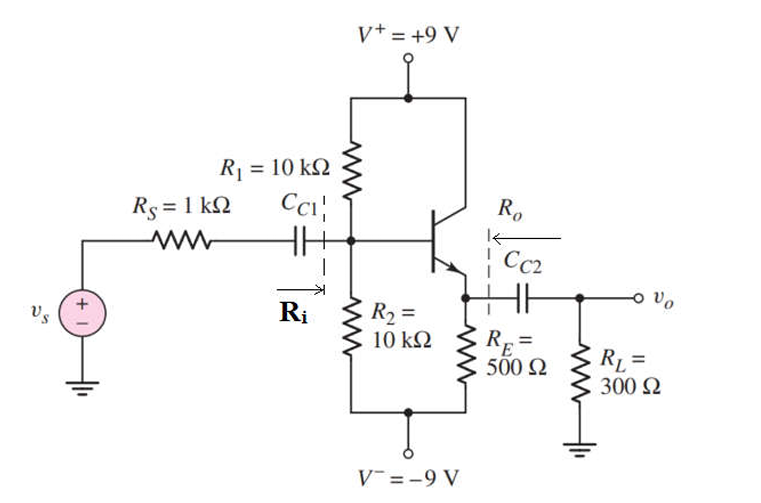
\includegraphics[width=.8\linewidth]{./my-chapters/my-images/Question3/debai.png}
\end{figure}

\answer{a}{Tìm điểm hoạt động $Q$ của BJT}

Xét hoạt động chế độ DC cho toàn mạch

\begin{figure}[H]
	\centering
	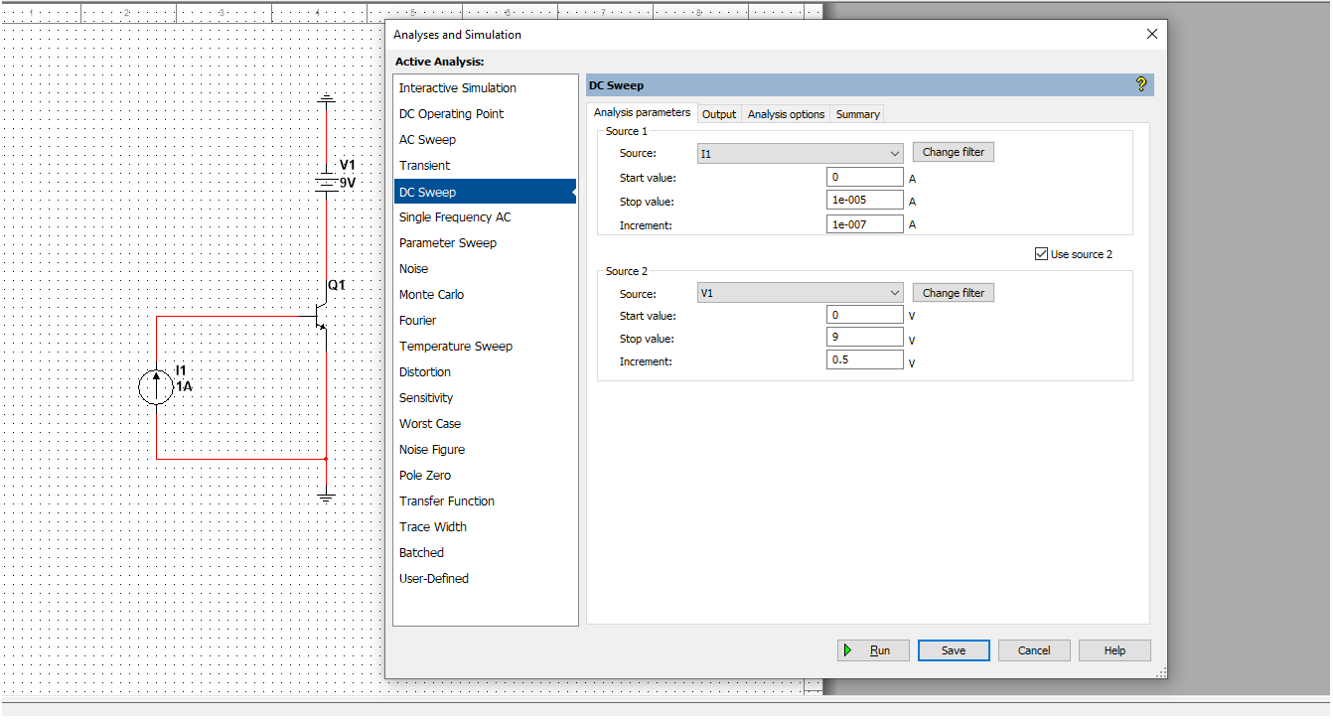
\includegraphics[width=.9\linewidth]{./my-chapters/my-images/Question3/a_timvbe.png}
	\caption{Tìm giá trị $V_{BE}$ của mạch.}
\end{figure}

Ta sử dụng chế độ DC Sweep để tìm giá trị $V_{BE}$ dẫn của mạch. Sau khi chạy tool, ta có kết quả như sau,

\begin{figure}[H]
	\centering
	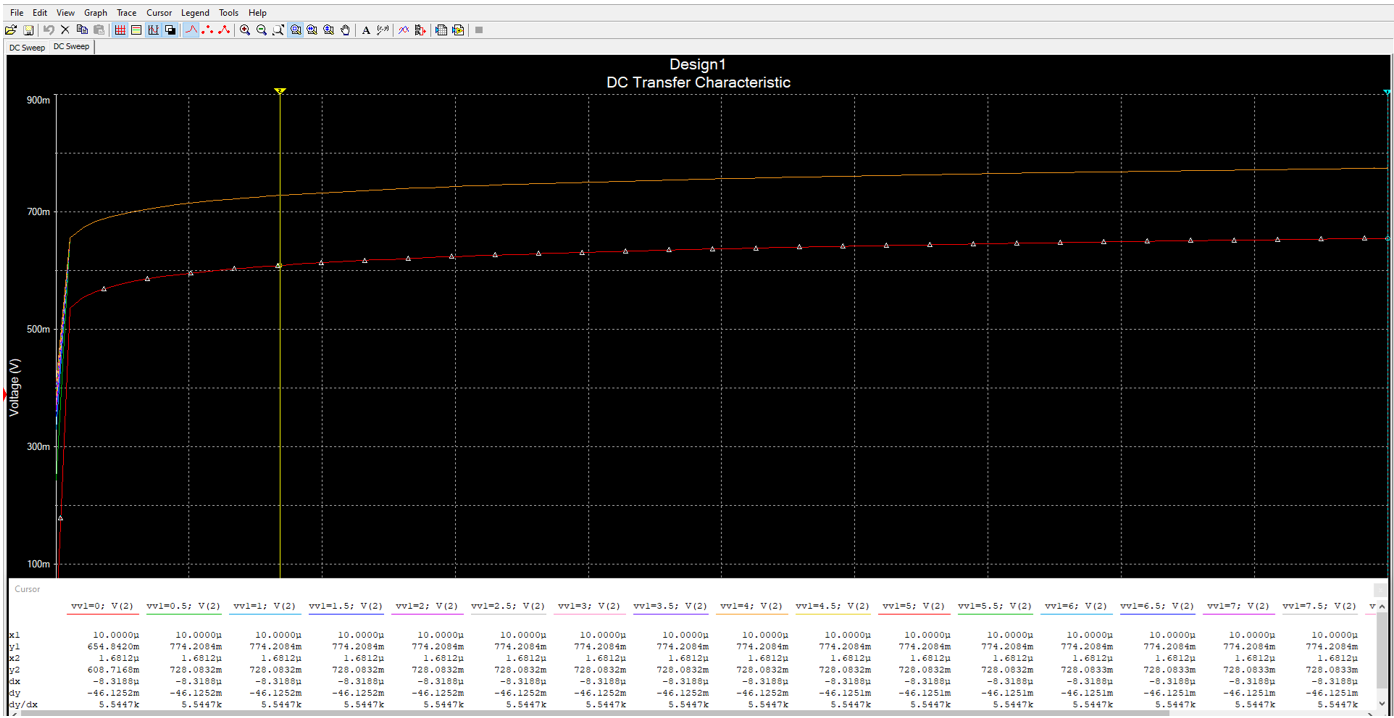
\includegraphics[width=.9\linewidth]{./my-chapters/my-images/Question3/a_giatriVbe.png}
	\caption{Kết quả sau khi chạy DC Sweep để tìm $V_{BE}$.}
\end{figure}

Như vậy, ta có giá trị điện áp $V_{BE}$ của BJT dẫn rơi vào tầm $\approx 0.774\,\textsf{mA}$.

\begin{itemize}[label=-]
	\item Tìm giá trị $I_{CQ}$
	
	\begin{figure}[H]
		\centering
		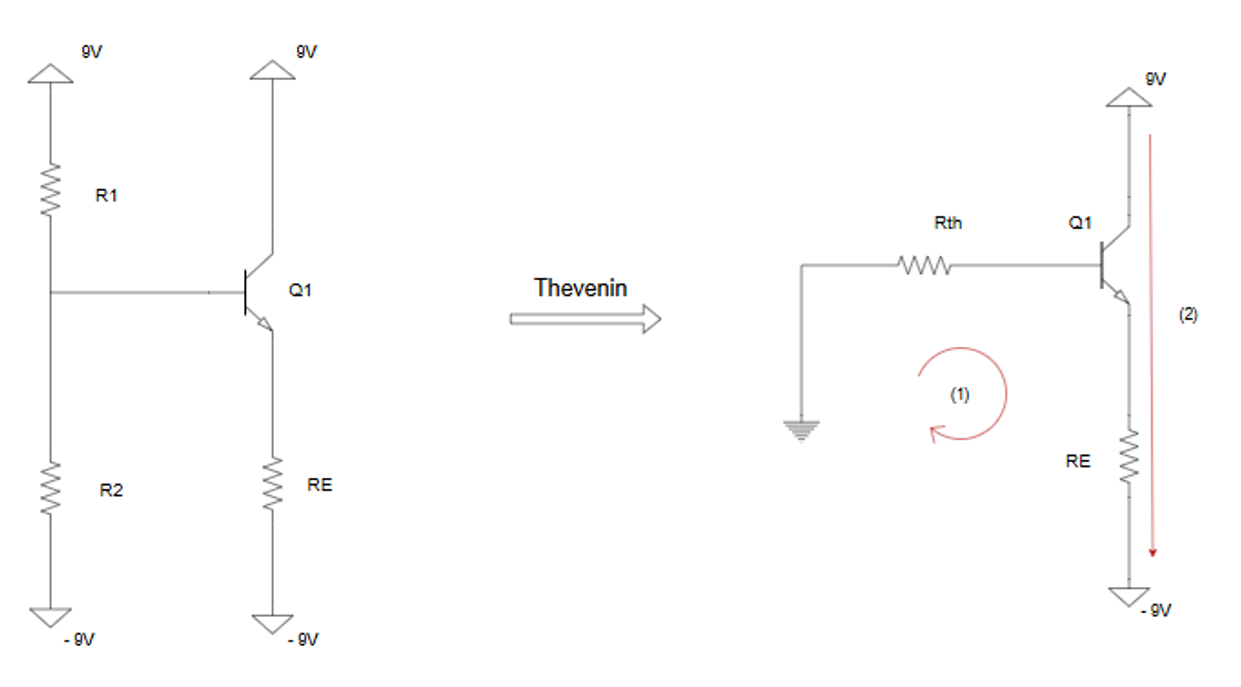
\includegraphics[width=.9\linewidth]{./my-chapters/my-images/Question3/a_thevenin.png}
	\end{figure}
	
	Thevenin ta có:
	\[ R_{th} = R_{1} // R_{2} = 5\,\textsf{k}\Omega \]
	\[ V_{th} = \dfrac{R_{2}}{R_{1} + R_{2}} V_{cc} - \dfrac{R_{1}}{R_{1} + R_{2}}V_{cc} = 0\,\textsf{V} \]
	
	Áp dụng KVL cho vòng (1):
	\[ I_{B}R_{th} + V_{BE} + I_{E}R_{E} - 9 = 0 \]
	Ta có: $I_E = (\beta + 1)I_B$
	\[
	\Longrightarrow I_B = \frac{9 - V_{BE}}{R_{th} + (\beta + 1)R_E}
	= \frac{9 - 0.774}{5 + (100 + 1)\times 0.5}
	= \frac{8.226}{55.5}
	= 0.148\,\text{mA}
	\]
	
	\[
	I_C = \beta I_B = 100 \times 0.148\ \text{mA}
	= 14.8\,\text{mA}
	\]
	
	\item Tìm giá trị $V_{CEQ}$
	
	Áp dụng KVL cho vòng (2):
	\[-9+V_{CE}+I_E R_E-9=0 \]
	Ta có: $I_C=\frac{\beta}{\left(\beta+1\right)}I_E$
	\[\Rightarrow V_{CE}=18-\frac{\left(\beta+1\right)}{\beta}I_C\times R_E=10.526\ V\]
	Vậy điểm làm việc Q của tầng 2 là : \finalresult{\left(I_{CQ},V_{CEQ}\right)=\left(14.8\ mA,10.526\ V\right)}.
	
	\item Kiểm tra kết quả
	
	\begin{figure}[H]
		\centering
		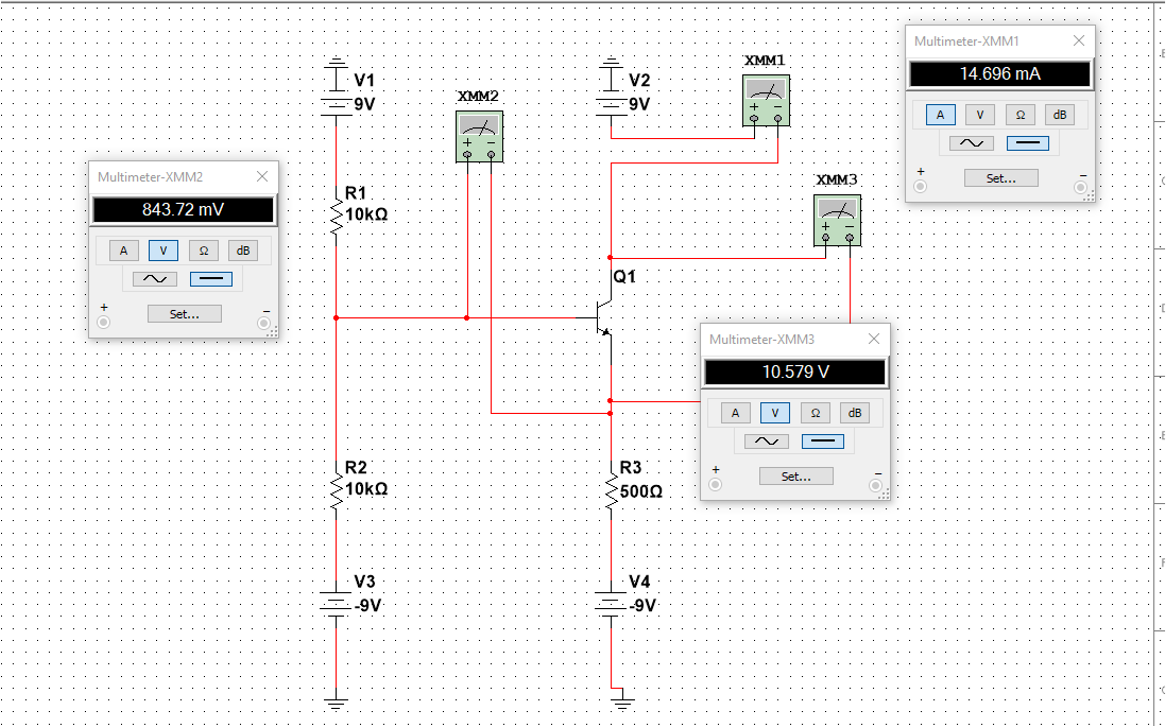
\includegraphics[width=\linewidth]{./my-chapters/my-images/Question3/a_ketqua.png}
	\end{figure}
\end{itemize}

\answer{b}{Đặt $v_s = V_s \sin\left(\omega t\right)$ vào mạch. Ngõ ra nối với tải $R_L = 1\,k\Omega$. Tìm $A_{vo}$, $G_v$, $R_i$, $R_o$ của mạch.}

Xét hoạt động chế độ AC cho toàn mạch:

\[
r_\pi = \frac{V_T}{I_B} = \frac{\beta V_T}{I_C} = 0.169\ k\Omega
\]

\[
r_o = \frac{V_A}{I_C} = \frac{100}{14.8} = 6.76\ k\Omega
\]

\[
A_{vo} = \frac{R_E}{\frac{r_\pi}{\beta + 1} + R_E} 
= \frac{0.5}{\frac{0.169}{101} + 0.5} 
= 0.997\ V/V
\]
$\Rightarrow$ \finalresult{A_{vo} = 0.997\,\textsf{V/V}}.

\[
R_{in} = R_1 // R_2 // (\beta + 1)\left(r_e + R_E // r_o\right) = 10k // 10k // 101 \times \left(\frac{r_\pi}{\beta + 1} + 500 // 6.76k\right)
= 4.52\ k\Omega
\]
$\Rightarrow$ \finalresult{R_{i} = 4.52\,\textsf{k}\Omega}.

\[
R_o = R_E // r_e // r_o 
= 0.5k // \frac{0.167k}{101} // 6.76k 
= 1.65\ \Omega
\]
$\Rightarrow$ \finalresult{R_{o} = 1.65\,\Omega}.

\[
G_v = \frac{R_{in}}{R_{in} + R_{sig}} \times 
\frac{R_L}{R_L + R_o} \times A_{vo} 
= \frac{4.52}{4.52 + 1} \times 
\frac{300}{300 + 1.65} \times 0.997 
= 0.81\ V/V
\]
$\Rightarrow$ \finalresult{G_{v} = 0.81\,\textsf{V/V}}.

Kiểm tra kết quả

\begin{figure}[H]
	\centering
	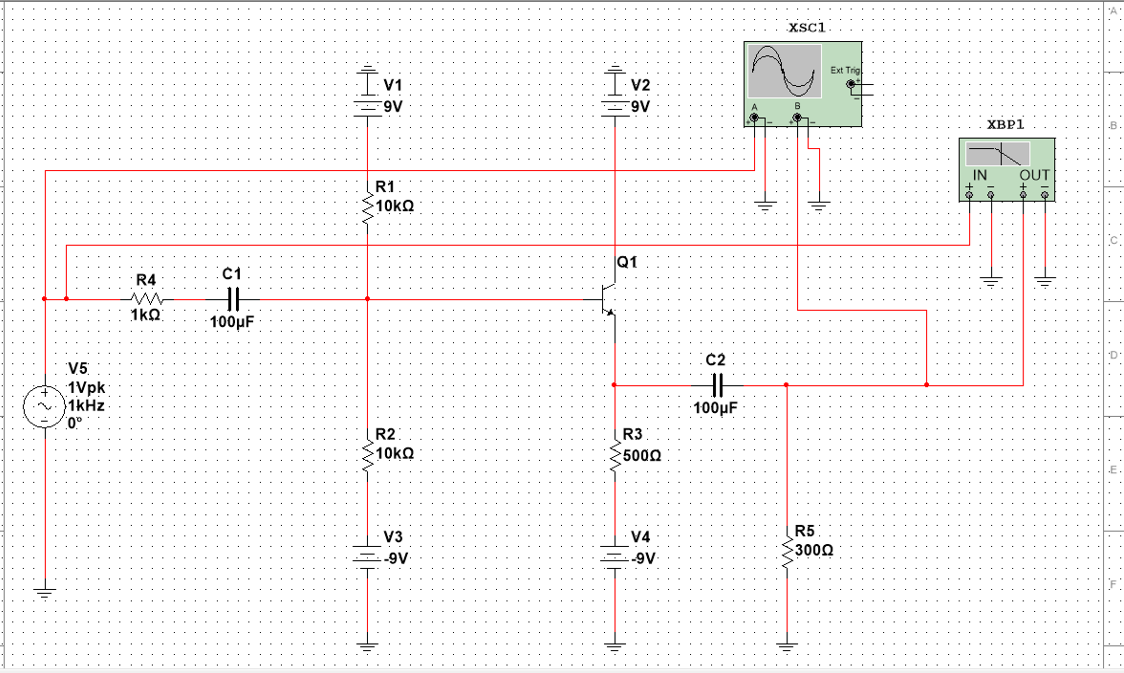
\includegraphics[width=\linewidth]{./my-chapters/my-images/Question3/b_dangsong.png}
	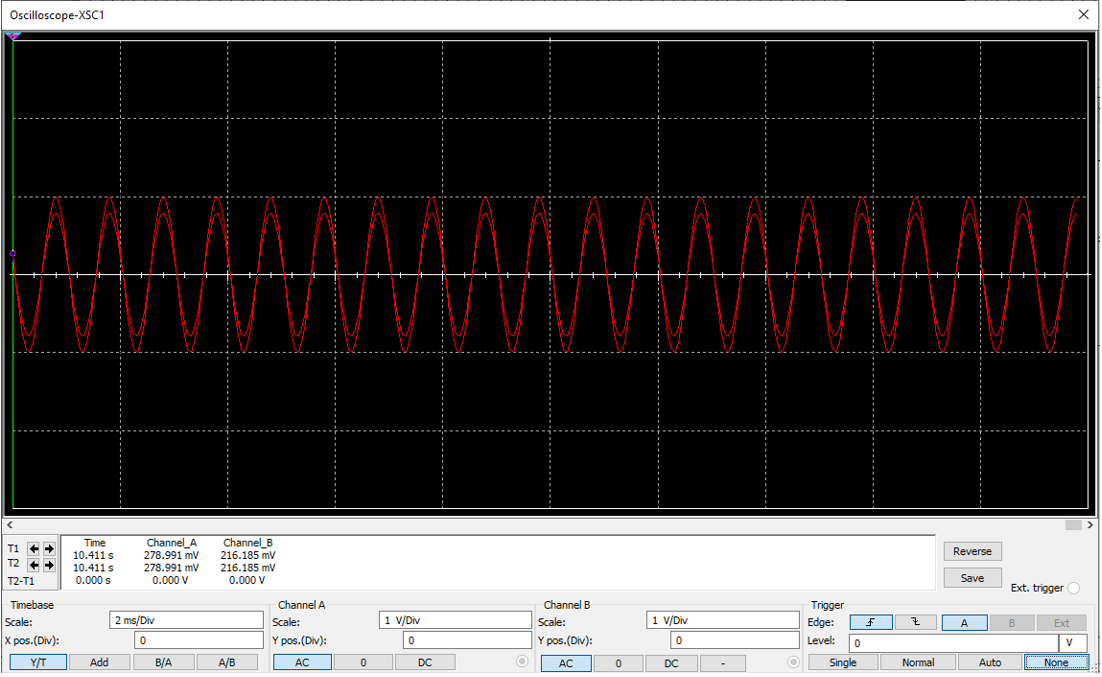
\includegraphics[width=\linewidth]{./my-chapters/my-images/Question3/b_dangwave.png}
	\caption{Dạng sóng ngõ vào và ngõ ra của mạch.}
\end{figure}

\begin{figure}[H]
	\centering
	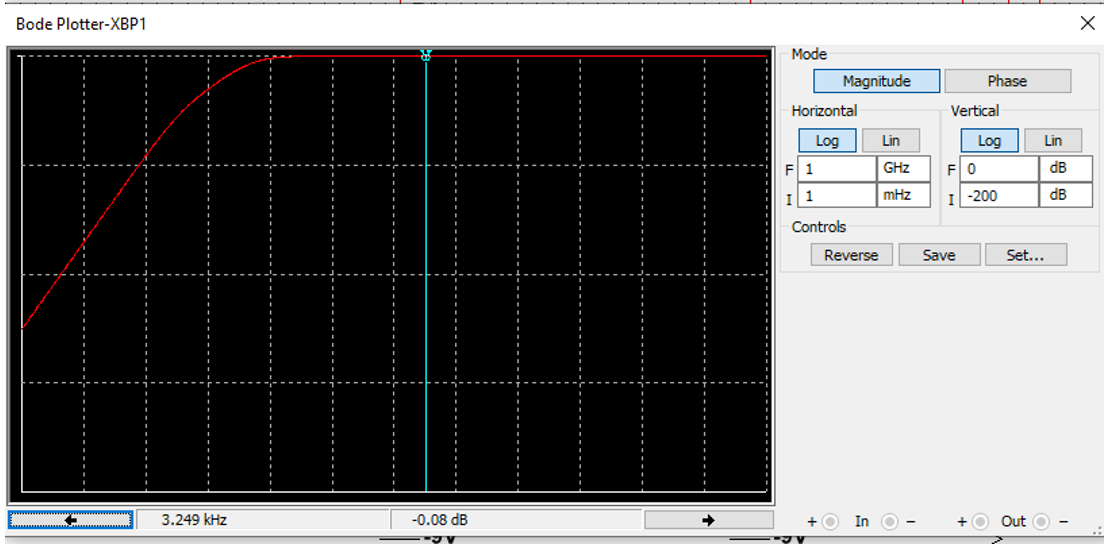
\includegraphics[width=\linewidth]{./my-chapters/my-images/Question3/a_vo.png}
	\caption{Tiến hành đo $A_{vo}\ =\ -0.08dB\ \approx\ 0.997\,\textsf{V/V}$.}
\end{figure}

\begin{figure}[H]
	\centering
	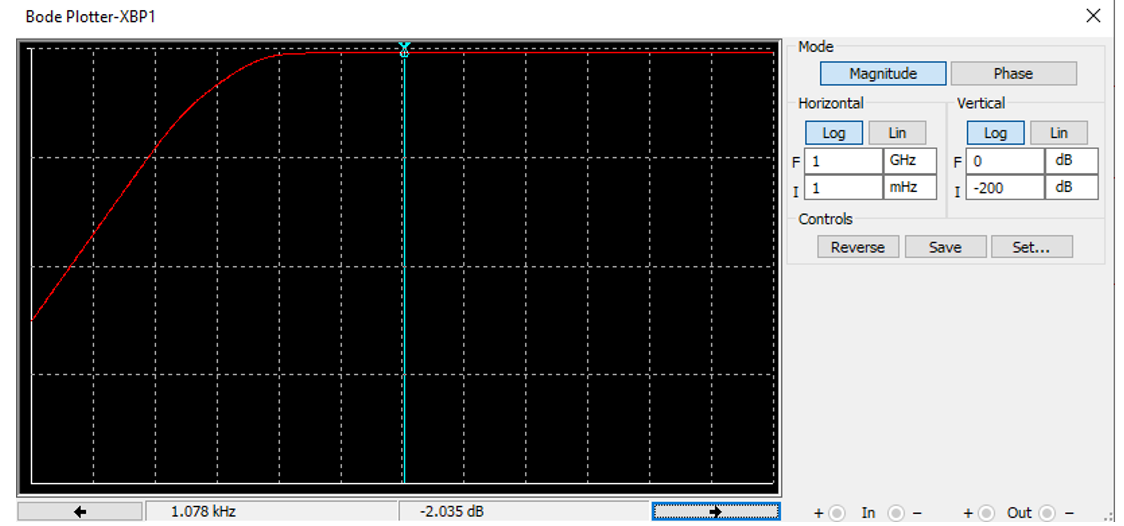
\includegraphics[width=\linewidth]{./my-chapters/my-images/Question3/b_gv.png}
	\caption{Tiến hành đo $G_{vo}\ =\ -2.035dB\ \approx\ 0.81\,\textsf{V/V}$.}
\end{figure}

\answer{c}{Tìm biên độ lớn nhất của $V_{m}$ để vs là tín hiệu nhỏ.}

Giả sử $V_{BE(on)}=0.7\,\textsf{V}$ và $V_{CE(sat)}=0.2\,\textsf{V}$. 

\textbf{Điểm chuyển từ Cut-off $\rightarrow$ Active của BJT:}
\[
V_{E}=V_{-}=-9\,\textsf{V} \;\Rightarrow\; V_{BE}=V_{BE(on)}=0.7\,\textsf{V}
\]
\[
\Rightarrow\; V_{i}=V_{E}+V_{BE(on)}=-9+0.7=-8.3\,\textsf{V}
\]

\textbf{Điểm chuyển từ Active $\rightarrow$ Saturation của BJT:}

$\text{BJT hoạt động trong vùng khuếch đại (active): } V_{BE}\approx0.7\,\textsf{V},\; V_{CE}>V_{CE(sat)}$

$\text{BJT đi vào vùng bão hòa khi: } V_{CE}=V_{CE(sat)}=0.2\,\textsf{V}$
\[
\Rightarrow\; V_{E}=V_{C}+V_{CE(sat)}=9-\left(-9\right)+0.2=18.2\,\textsf{V}
\]
\[
V_{i}=V_{E}+V_{BE(on)}=18.2+0.7=18.9\,\textsf{V}
\]

Kiểm tra kết quả

\begin{figure}[H]
	\centering
	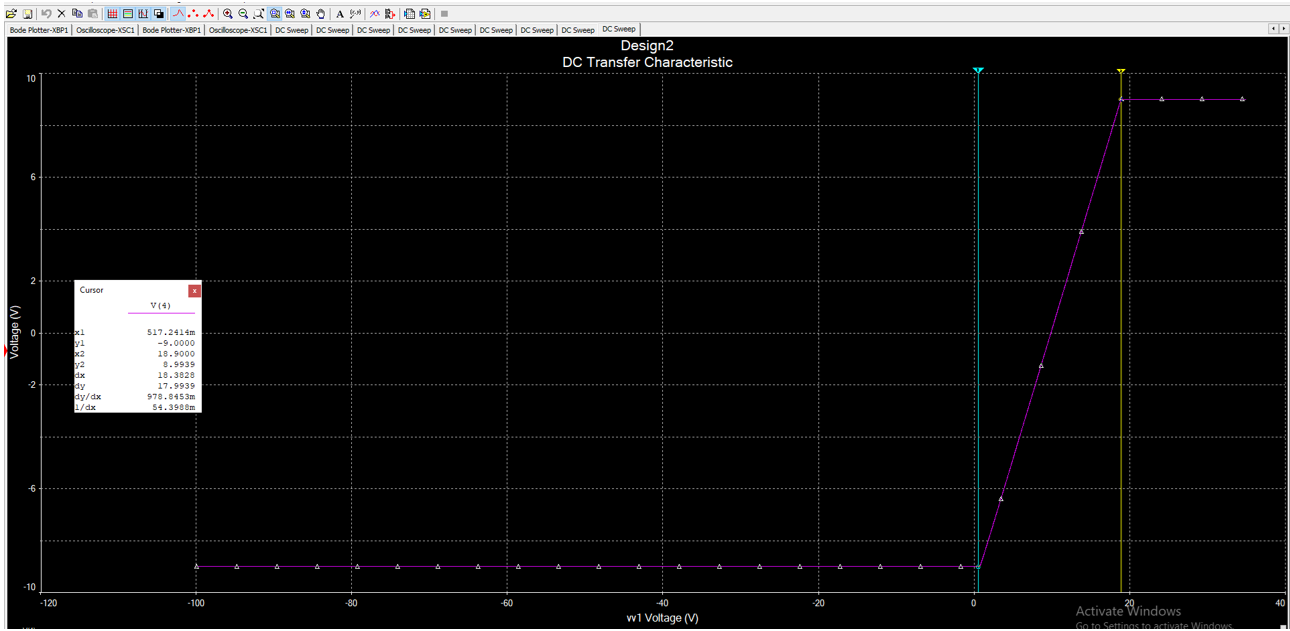
\includegraphics[width=.9\linewidth]{./my-chapters/my-images/Question3/c_ketqua.png}
\end{figure}

\answer{d}{Lựa chọn các tụ $C_{C1}$, $C_{C2}$ để mạch có $f_{L}=100Hz$.}

\begin{itemize}[label=-, leftmargin=2cm]
	\item \textbf{Xét ảnh hưởng của tụ \( C_1 \):}
	\[
	R_{C_1} = R_{in}
	\quad \Longrightarrow \quad
	\omega_{p_1} = \frac{1}{C_1 R_{in}}
	\]
	
	\item \textbf{Xét ảnh hưởng của tụ \( C_2 \):}
	\[
	R_{C_2} = R_E // R_L
	\quad \Longrightarrow \quad
	\omega_{p_2} = \frac{1}{C_2 (R_E // R_L)}
	\]
	
	\item Theo phương pháp cực tần số trội (\emph{dominant pole}), chọn \( C_1 \) tạo cực trội ở 
	\( f_{C_1} = 100\,\text{Hz} \), 
	và \( C_2 \) tạo cực ở \( f_{C_2} = 10\,\text{Hz} \).  
	Tần số cắt của mạch:
	\[
	f_L = \sqrt{f_{C_1}^2 + f_{C_2}^2}
	\]
	
	\item \textbf{Lựa chọn các tụ \( C_1, C_2 \):}
	
	$\Rightarrow$ \finalresult{C_1 = \frac{1}{2\pi \times 100 \times (4.52k)} = 0.35\,\mu F}.
	
	$\Rightarrow$ \finalresult{C_2 = \frac{1}{2\pi \times 10 \times (500 // 300)} = 84.88\,\mu F}.
\end{itemize}

Kiểm tra kết quả

\begin{figure}[H]
	\centering
	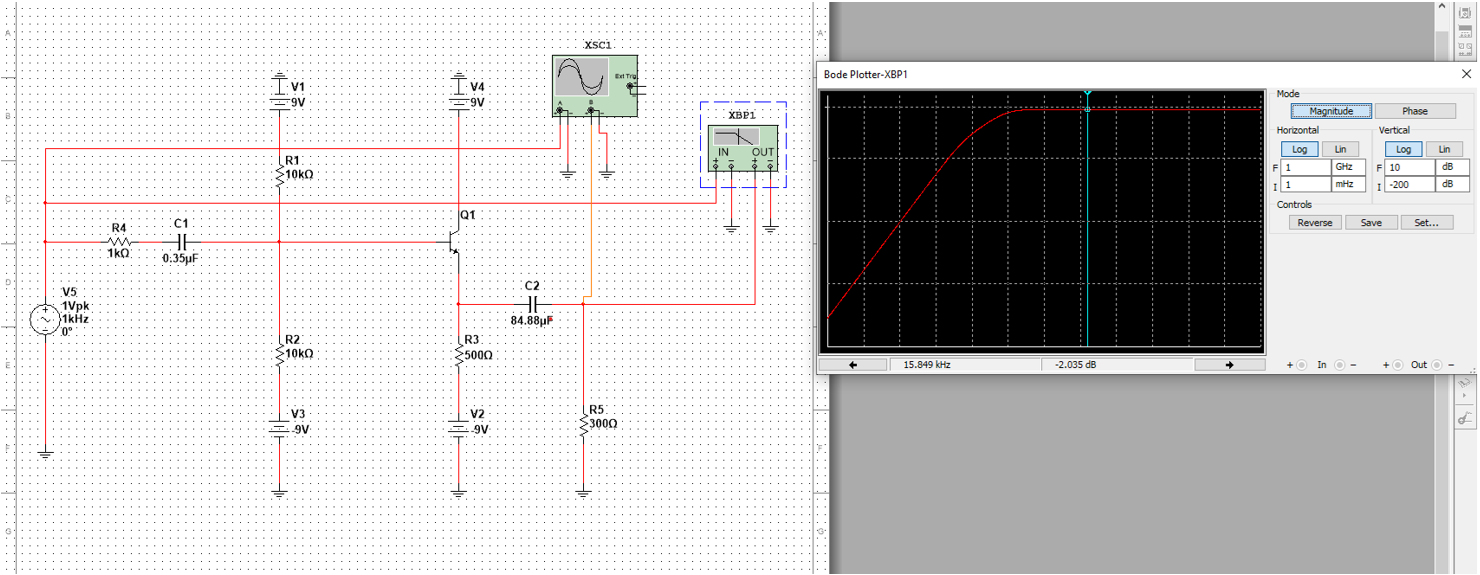
\includegraphics[width=.9\linewidth]{./my-chapters/my-images/Question3/d_ketqua.png}
\end{figure}

